\section{Analyse des Krebsnebels}
\label{sec:analyse}

\subsection{Ablauf einer stereoskopischen MAGIC Analyse}

Abbildung~\ref{fig:analysischain} zeigt den typischen Ablauf einer
stereoskopischen Analyse mit MAGIC Daten. Die hierzu verwendeten einzelnen
Softwarepakete sind eingebettet in das MARS Framework. In einem ersten Schritt
werden die Rohdaten der beiden Teleskope einzeln vorprozessiert. Dazu gehören
die Zeit- und Ladungskalibrierung der einzelnen Pixel der Kamera (sorcerer),
sowie das image cleaning und die Parametrisierung des Kamerabildes (star).
Im Anschluss daran werden die Daten der Teleskope durch die Software superstar
kombiniert und Stereoparameter berechnet. 

\begin{figure}
  \centering
  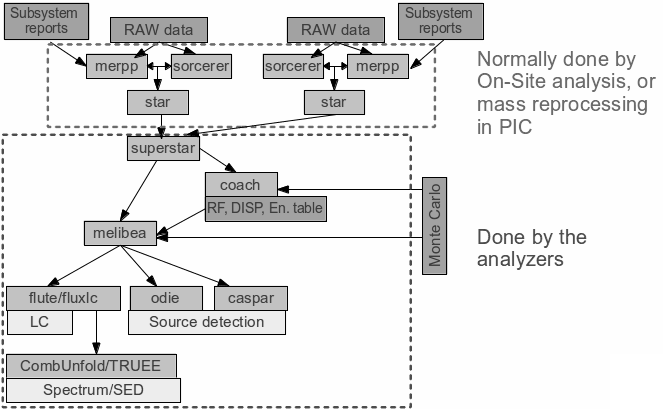
\includegraphics[width=0.9\textwidth]{figures/analysischain.png}
  \caption{Ablauf einer typischen stereoskopischen Analyse. Zunächst werden die
  Rohdaten der beiden Teleskope einzeln vorprozessiert und dann durch die
  Software superstar kombiniert. [...]}
  % Referenz: MAGIC wiki
  \label{fig:analysischain}
\end{figure}

\subsection{Wahl der Analyseparameter}

\subsection{Ergebnisse}
